\section{Assembling boundary integral operators with OpenCL}

In this section we discuss in more detail the assembly of boundary integral operators with OpenCL
and how we integrated this into our Python workflow. We start with a brief introduction to OpenCL and then
dive into how we use OpenCL as part of Bempp-cl.

\subsection{What is OpenCL?}

OpenCL (\url{https://www.khronos.org/opencl/}) is a heterogeneous compute standard for CPUs, GPUs, FPGAs, and other types of devices that provide conformant drivers. At its core OpenCL executes compute kernels that can be written in C99, or more recently, in C++. The current version of OpenCL is 3.0, though the most widely implemented standard is OpenCL 1.2, which Bempp-cl uses. OpenCL splits the computational tasks into work-items, each of which represents a single execution of a compute kernel. Work items are grouped together into work-groups, which share local memory. Barrier synchronisation is only allowed within a work-group. All work-items are uniquely indexed by a one, two, or three dimensional index space, called NDRange. Kernels are launched onto a compute device (e.g. CPU or GPU) from a host device. OpenCL allows kernels to be loaded as strings and compiled on the fly for a given device, making it well suited for launching from high-productivity languages. To launch an OpenCL kernel the following steps need to be performed.
\begin{itemize}
	\item Initialise buffers on the compute device.
	\item Compute relevant data from host to the compute device.
	\item Load a kernel string and just-in-time compile it for the device.
	\item Execute the kernel for the given buffers and chosen index space.
	\item Copy results back to the host.
\end{itemize}
An excellent feature of OpenCL is its very good support for vectorised operations. OpenCL provides vector data types, such as \textbf{double4}, that can hold four double values in a SIMD register and defines a number of standard operations for these vector types. This makes it easy to explicitly target modern SIMD execution in a portable way while avoiding difficult compiler intrinsics and keeping kernel code readable.

Python has excellent OpenCL support through the PyOpenCL library by Andreas Kloeckner, which automates much of the initialisation of the OpenCL environment and makes it easy to create buffers and launch OpenCL kernels from Python.

\subsection{OpenCL Assembly in Bempp-cl}

\begin{figure*}
	\center
	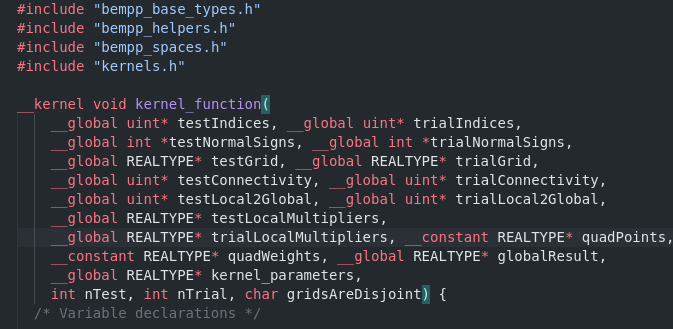
\includegraphics[width=12cm]{img/kernel_header}
	\caption{Definition of the OpenCL compute kernel for scalar integral equations.}
	\label{fig:kernel_definition}
\end{figure*}


Bempp-cl has OpenCL kernels for all its boundary operators. All operators have the same interface and are launched in the same way. In the first step the relevant data will need to be copied to the compute device. This data consists of:

\begin{itemize}
	\item Test and trial indices of triangles over which to be integrated.
	\item Signs of the normal directions for the spaces.
	\item Test and trial grid as flat floating point array, defining each triangle through nine floating point numbers, specifying the $(x, y, z)$ coordinates of each of the three nodes of a triangle.
	\item Test and trial connectivity information that stores the indices of each node for each triangle.
	\item Test and trial mappings of local triangle degrees of freedom to global degrees of freedom.
	\item Test and trial basis function multipliers for each triangle.
	\item Quadrature points and quadrature weights.
	\item A buffer that contains the global assembled matrix.
	\item Additional kernel parameters, such as the wavenumber for Helmholtz problems.
	\item Number of test and trial degrees of freedom.
	\item A single byte that is set to one if the test and trial grids are disjoint.
\end{itemize}
The actual kernel definition is shown in Figure \ref{fig:kernel_definition}.
Before the kernel can be launched, it needs to be configured and just-in-time compiled. Kernel configuration happens through C-style preprocessor definitions that are passed through the just-in-time compiler. These include the names of the test and trial space, the name of the function that evaluates the integral kernel, choosing between single and double precision types, and for SIMD enhanced kernel the vector length of the SIMD types.
For example, in Figure \ref{fig:kernel_definition} all floating point types have the name REALTYPE. This is substituted with either \textit{float} or \textit{double} during just-in-time compilation.

Each work-item computes via numerical quadrature all interactions via the integral kernel of basis functions on the trial element with basis functions on the test element. Before summing the result into the global result buffer, the kernel checks via the connectivity information if the test and trial triangle are adjoint or identical. For this it simply checks if at at least one of the node indices of the test triangle is identical to one of the node indices of the trial triangle. If this is true and the grids are not disjoint, the result of the kernel is discarded and not summed back into the global result buffer. The reason is that for adjoint triangles a separate singular quadrature rule is used. The effect is that a few work-items do work that is discarded. However, in a grid with $N$ elements the number of triangle pairs requiring a singular quadrature rule is $\mathcal{O}(N)$, while the total number of interactions is $N^2$. Hence, only a tiny fraction of work-items are discarded.

\subsection{SIMD optimized kernels}

The above description was valid for kernels that do not take advantage of CPU SIMD operations are kernels that run directly on a GPU device. For SIMD optimisation on CPUs we proceed slightly differently. The corresponding kernel in principle works as described above, but batches together the interaction on one test triangle with X trial triangles, where X is either 4, 8, or 16, depending on the number of available SIMD lanes. This strategy allows us to optimise almost all floating point operations within a kernel run for SIMD operation. If the number of trial elements is not divisible by 4, 8, or 16, then the few remaining trial elements are assembled with the standard-non vectorised kernel.

Each kernel definition is stored in two variants, one with the ending \textit{\_novec.cl} and another one with the ending \textit{\_vec.cl}. The vectorised variant is configured via preprocessor directives for the desired number of vector lanes. Having to develop two OpenCL kernel codes for each operator is a certain amount of overhead. If we write a new kernel, we first implement the non-vectorised version. Then, with the help of preprocessor directives and a number of helper functions that do the actual implementation of operations depending on whether the kernel is vectorised or not, it is usually a matter of an hour or two to convert the non-vectorised kernel into a vectorised version.

Alternatively, some CPU OpenCL runtime environments have the option to try and auto-vectorise kernels by batching together work items on SIMD lanes, similarly to what we do manually. In our experience this works well for very simple kernels but often fails for more complex OpenCL kernels. This is why we decided to implement this strategy manually.

A completely different SIMD strategy is based on batching together quadrature evaluations within a single test/triangle pair. There are two disadvantages to this approach. First, it only works well if the number of quadrature points is a multiple of the available SIMD lanes. Second, other operations such as the geometry calculations for each element then can not be SIMD optimized as these are only performed once per test/triangle pair.


\subsection{Assembling the singular part of integral operators}

The assembly of the singular part of an integral operator works a bit differently. Remember that the singular part consists of triangle parts which are adjacent to each other or identical. There are $\mathcal{O}(N)$ of such pairs. We are using fully numerical quadrature rules for these integrals that are based on subdividing the four-dimensional integration domain and using transformation techniques to remove the singularities. This gives highly accurate evaluations of these integration pairs but requires a large number (typically over $1000$) quadrature points per triangle pair. Hence, we create one workgroup for each triangle pair and inside this workgroup have a number of work-items that are evaluating the quadrature rules and then at the end sum up the result together. Depending on how two triangles are in relationship to each other different types of singular quadrature rules are needed. We solve this pre-loading all possible quadrature rules onto the device and also store for each triangle pair an index into the required quadrature rule so that the kernel function can select the correct rule to evaluate. For the singular quadrature rules we did not implement separate SIMD optimized kernels as the proposed implementation is already highly efficient and requires only a fraction of the computational time of the regular quadrature rules described above. At the end, the singular integral values are either summed into the overall result matrix, or if desired by the user, stored as separate sparse matrix.

\section{Numba assembly of integral operators}

The Numba assembly of integral operators is structured differently from the OpenCL assembly. In OpenCL we create a large number of work-items that are executed in parallel on the compute device by the runtime system with the details of the parallel execution left to the device driver. For Numba we use classical loop based parallelism. Each loop iteration is the assembly of one test element with all trial elements. Within each loop we partially optimized for SIMD instruction, though this depends on the autovectorization of the just-in-time compiler and cannot be explicitly targeted in Numba. Again, we separate regular and singular interactions. In the next section we give some more details on SIMD optimization in Numba at the example of the Laplace kernel.

\section{SIMD optimized evaluation of the Laplace kernel with Numba}
